\documentclass{article}
\usepackage[utf8]{inputenc}
\usepackage{tikz}
\usepackage{tikz-feynman}
\usepackage{color}
\usetikzlibrary{decorations.pathmorphing}
\tikzset{snake it/.style={decorate, decoration=snake}}

\begin{document}
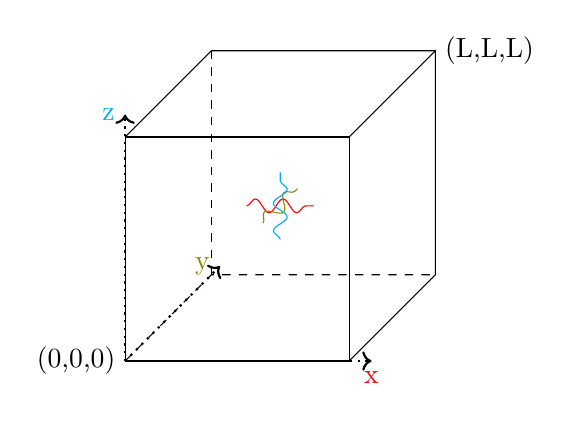
\begin{tikzpicture}

\draw (0,0,0) node[anchor=east]{(0,0,0)}  -- (1mm,0,0) -- (1mm,1mm,0) -- (0,1mm,0) -- cycle;
\draw (1mm,0,0) -- (1mm,0,-1mm) -- (1mm,1mm,-1mm) -- (1mm,1mm,0);
\draw (1mm,1mm,-1mm) node[anchor=west]{(L,L,L)} -- (0,1mm,-1mm) -- (0,1mm,0);

\draw[dashed](0,0,0) -- (0,0,-1mm) -- (1mm,0,-1mm);
\draw[dashed](0,0,-1mm) -- (0,1mm,-1mm);

\draw[dotted, thick, ->](0,0,0) -- (1.1mm,0,0) node[text=red, anchor=north]{x};
\draw[dotted, thick,->](0,0,0) -- (0,0,-1.1mm) node[text=olive, anchor=east]{y};
\draw[dotted, thick,->](0,0,0) -- (0,1.1mm,0) node[text=cyan, anchor=east]{z};

\path [draw=red,snake it]
    (0.35mm,0.5mm,-0.5mm) --  (0.65mm,0.5mm,-0.5mm);
\path [draw=olive,snake it]
    (0.5mm,0.5mm,-0.3mm) --  (0.5mm,0.5mm,-0.7mm);
\path [draw=cyan,snake it]
    (0.5mm,0.35mm,-0.5mm) --  (0.5mm,0.65mm,-0.5mm);

\end{tikzpicture}

\end{document}